\section{Software Setup}
The software setup of the system is presented in the following sections, and will explain all the software setup done on the Raspberry Pi in detail. Most of the setup information; which dependencies and what packages are needed obtained from the PyImageSearch website\cite{pis}.\\

I will present different code examples in this and the next section, which will consist of Python code and Bash (Unix Shell) code. The bash code will be presented as a runnable script in the Raspberry Pi shell like this:
\begin{minted}[frame=lines,framesep=2mm]{bash}
$ sudo apt-get install <SomeSoftware>
\end{minted}
These commands are mostly used to install the needed framework and dependencies for the application in Python. \\

The Python code examples will be presented in the following manner:
\begin{minted}[frame=single,framesep=2pt,linenos]{python}
#This program prints Hello, world!
print('Hello, world!')
\end{minted}

\subsection{Operating System, Raspbian Jessie}
The operating system installed on the Raspberry Pi is Raspbian Jessie. This is the most widely used OS for the Raspberry Pi, and provides all I need to make the application work. Keep in mind this OS is chosen as a high-level test platform for my application, to see if it is feasible to implement the algorithm. Raspian Jessie features a GUI similar to Ubuntu and is easy to use.\\

The idea is to show the feasibility of the implementation on a high-level OS, then gradually optimize the implementation by using a headless OS and a better optimized programming language.

\subsubsection{Installation}
There are a few steps required to install Raspbian Jessie. Most of the information is found online, and is easily available. There are a few components needed to install the Raspbian Jessie OS.\\

Requirements:
\begin{itemize}
\item SD Card with at least 8GB
\item SD Card reader
\item Image writing software tool
\end{itemize}

To install an OS on the Raspberry Pi:
\begin{enumerate}
\item Download the Raspbian Jessie image\cite{jessie}
\item Insert the SD Card into the SD Card reader on a computer
\item Download and install Win32DiskImager\cite{win}
\item Select the OS image and Write to the SD Card
\end{enumerate}

The SD Card now contains the OS needed to run on the Raspberry Pi. The Raspberry Pi boots from the SD Card inserted in the card reader automatically, so simply insert the SD Card in the reader on the Raspberry Pi and plug in the power source. 

\subsection{Python 2.7}
The system has been implemented in Python 2.7. This choice was based on the compatibility with OpenCV, which is supported by Python and C++, and the fact that there exists many image processing implementation projects for the Raspberry Pi in Python.\\

Python is a high-level programming language that is used for general-purpose programming. It is an interpreted language which features a strong focus on code readability and is an expressive language that often lets programmers express functionality in fewer lines than in for instance C++. \cite{gui}

\subsubsection{Installation}
The development version of the Python header files needs to be installed so I can compile OpenCV with Python bindings later:
\begin{minted}[frame=lines,framesep=2mm]{bash}
$ sudo apt-get install python2.7-dev
\end{minted}
This is so I do not run into errors when running \emph{make} to compile OpenCV later. I also need to install 'pip', a Python package manager:
\begin{minted}[frame=lines,framesep=2mm]{bash}
$ wget https://bootstrap.pypa.io/get-pip.py
$ sudo python get-pip.py
\end{minted}

%%%%%%%%%%%%%%%%%%%%%%%%%%
\subsubsection{Dependencies}
Before installing the Virtual Environment in the next section, some dependencies needed for the application needs to be installed. First off update and upgrade the Raspberry Pi to be sure all the packages are up to date:
\begin{minted}[frame=lines,framesep=2mm]{bash}
$ sudo apt-get update
$ sudo apt-get upgrade
\end{minted}
Cmake needs to be installed so OpenCV can be compiled.
\begin{minted}[frame=lines,framesep=2mm]{bash}
$ sudo apt-get install build-essential cmake pkg-config
\end{minted}
Install image and video I/O packages for Image processing:
\begin{minted}[frame=lines,framesep=2mm,breaklines]{bash}
$ sudo apt-get install libjpeg-dev libtiff5-dev libjasper-dev libpng12-dev
$ sudo apt-get install libavcodec-dev libavformat-dev libswscale-dev libv4l-dev
$ sudo apt-get install libxvidcore-dev libx264-dev
\end{minted}
Install some OpenCV dependencies:
\begin{minted}[frame=lines,framesep=2mm]{bash}
$ sudo apt-get install libgtk2.0-dev
$ sudo apt-get install libatlas-base-dev gfortran
\end{minted}


%%%%%%%%%%%%%%%%%%%%%%%%%
\subsubsection{Virtual Environment}
It is good practice to incorporate and utilize virtual environments to keep the dependencies required by different projects in separate places. This creates isolated, independent Python environments for each of the projects. This will make it easy to keep track of all the dependencies needed in the application. To install:
\begin{minted}[frame=lines,framesep=2mm]{bash}
$ sudo pip install virtualenv virtualenvwrapper
$ sudo rm -rf ~/.cache/pip
\end{minted}
Update the \textbf{$\sim$/.profile} file with the following script:
\begin{minted}[frame=lines,framesep=2mm]{bash}
$ echo -e "\n# virtualenv and virtualenvwrapper" >> ~/.profile
$ echo "export WORKON_HOME=$HOME/.virtualenvs" >> ~/.profile
$ echo "source /usr/local/bin/virtualenvwrapper.sh" >> ~/.profile
\end{minted}
This will update the \textbf{$\sim$/.profile} file so that the virtual environment can be accessed. After this I can create the virtual environment, which I will call 'cv', for Python:
\begin{minted}[frame=lines,framesep=2mm]{bash}
$ mkvirtualenv cv -p python2
\end{minted}
I can now install and develop the project entirely independent from any other Python projects on the Raspberry Pi. To work on the virtual environment use the following command:
\begin{minted}[frame=lines,framesep=2mm]{bash}
$ source ~/.profile
$ workon cv
\end{minted}
When working in the virtual environment, the shell will display '(cv)' on the left side of the command prompt like this:
\begin{minted}[frame=lines,framesep=2mm]{bash}
(cv) pi@raspberrypi:~ $ <command>
\end{minted}
From this point on in the software setup, it is assumed that I will be working in the virtual environment. For numerical processing, I need to install a Python package named Numpy:
\begin{minted}[frame=lines,framesep=2mm]{bash}
$ pip install numpy
\end{minted}
This installation can take up to 10 minutes to finish.

\subsection{OpenCV 3}
Open Source Computer Vision (OpenCV) is an open-source image processing toolbox used for computer vision applications, often in real-time\cite{opencv}. It features a library of image processing functions similar to that of the Image Processing Toolbox™ in MATLAB. 
%litt mer

\subsubsection{Installation and Compilation}
Grab the official OpenCV software with the latest verison (April 2017 - 3.2.0) from their Github repository. 
\begin{minted}[frame=lines,framesep=2mm]{bash}
$ cd ~
$ wget -O opencv.zip https://github.com/Itseez/opencv/archive/3.2.0.zip
$ unzip opencv.zip
\end{minted}
For some extra features I install the full version of OpenCV, by accessing the opencv\_contrib repository:
\begin{minted}[frame=lines,framesep=2mm,breaklines]{bash}
$ wget -O opencv_contrib.zip https://github.com/Itseez/opencv_contrib/archive/3.2.0.zip
$ unzip opencv_contrib.zip
\end{minted}
After the download has finished, the compilation of OpenCV can be started. First I need to be working in (cv) virtual environment:
\begin{minted}[frame=lines,framesep=2mm]{bash}
$ workon cv
\end{minted}
After this, CMake can be run to setup OpenCV:
\begin{minted}[frame=lines,framesep=2mm]{bash}
$ cd ~/opencv-3.2.0/
$ mkdir build
$ cd build
$ cmake -D CMAKE_BUILD_TYPE=RELEASE \
    -D CMAKE_INSTALL_PREFIX=/usr/local \
    -D INSTALL_PYTHON_EXAMPLES=ON \
    -D OPENCV_EXTRA_MODULES_PATH=~/opencv_contrib-3.2.0/modules \
    -D BUILD_EXAMPLES=ON ..
\end{minted}
The output of the CMake should be inspected to make sure the Python 2.7 make location is in the virtual environment (cv). If this is the case, I can make:
\begin{minted}[frame=lines,framesep=2mm]{bash}
$ make
\end{minted}
This will compile OpenCV with one core of the CPU. Some attempts was done with the command 'make -j4' which utilizes all four cores of the CPU. This was not successful, and made the Raspberry Pi crash in all attempts. This operation takes over one hour. After the compilation is finished, the next step is to install:
\begin{minted}[frame=lines,framesep=2mm]{bash}
$ sudo make install
$ sudo ldconfig
\end{minted}
The final step is to link the bindings of OpenCV into the virtual environment:
\begin{minted}[frame=lines,framesep=2mm]{bash}
$ cd ~/.virtualenvs/cv/lib/python2.7/site-packages/
$ ln -s /usr/local/lib/python2.7/site-packages/cv2.so cv2.so
\end{minted}
All the OpenCV functionality is now usable in the virtual environment, and opens up image processing functionality in Python. To use OpenCV in Python projects, include it at the start of the program:
\begin{minted}[frame=single,framesep=2pt,linenos]{python}
#OpenCV
import cv2
#Numpy
import numpy

#Rest of program
\end{minted}

\subsection{Remote Desktop and Connection}
I found it beneficial to be able to work remotely on the Raspberry Pi from my workplace in a remote desktop. This means I can run the Raspberry Pi headless when testing the image processing application. The steps involved in connecting to the Raspberry Pi is the following:
\begin{enumerate}
\item Determine the Raspberry Pi IP address
\item Connect through the "Remote Desktop Connection" application in Windows
\end{enumerate}

\subsubsection{Determining IP address}
I have installed Samba on the Raspberry Pi, so that the device can be pinged on the local network to obtain the IP address:
\begin{minted}[frame=lines,framesep=2mm]{bash}
$ sudo apt-get install samba
\end{minted}
By typing the following command in the Windows cmd Shell, it returns the IP address of the Raspberry Pi:
\begin{minted}[frame=lines,framesep=2mm]{bash}
ping raspberrypi
\end{minted}
This will output:
\begin{figure}[H]
  \centering
  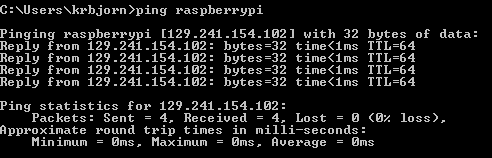
\includegraphics[width=1\textwidth]{fig/ping}
  \caption{Raspberry Pi IP}
  \label{fig:ping}
\end{figure}

\subsubsection{Remote Desktop}
To connect remotely to the Raspberry Pi, I have installed some dependencies that make this work:
\begin{minted}[frame=lines,framesep=2mm]{bash}
$ sudo apt-get install xrdp
$ sudo apt-get install tightvncserver
\end{minted}
Now that I have the Raspberry Pi IP address, I can connect to it through the Remote Desktop Connection application in Windows, by typing in the Raspberry Pi IP address in the following window:
\begin{figure}[H]
  \centering
  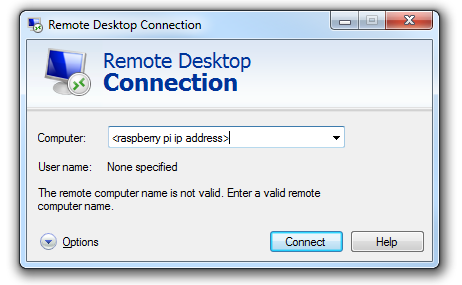
\includegraphics[width=0.6\textwidth]{fig/remote1}
  \caption{Windows Remote Desktop Connection}
  \label{fig:remote1}
\end{figure}
This will open a new window that asks for a username and password for the Raspberry Pi. The username and password is:
\begin{table}[H]
\centering

\begin{tabular}{|l|l|}
\hline
\textbf{Username}        & \textbf{Password}               \\ \hline
\multicolumn{1}{|c|}{pi} & \multicolumn{1}{c|}{master2017} \\ \hline
\end{tabular}
\caption{Username and Password}
\label{password}
\end{table}
After entering the username and password in this login prompt, I have complete remote access to the Raspberry Pi.
\begin{figure}[H]
  \centering
  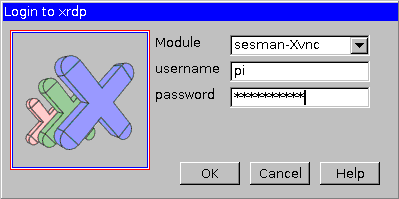
\includegraphics[width=0.6\textwidth]{fig/remote2}
  \caption{Raspberry Pi Login}
  \label{fig:ping}
\end{figure}










